
%% bare_jrnl.tex
%% V1.3
%% 2007/01/11
%% by Michael Shell
%% see http://www.michaelshell.org/
%% for current contact information.
%%
%% This is a skeleton file demonstrating the use of IEEEtran.cls
%% (requires IEEEtran.cls version 1.7 or later) with an IEEE journal paper.
%%
%% Support sites:
%% http://www.michaelshell.org/tex/ieeetran/
%% http://www.ctan.org/tex-archive/macros/latex/contrib/IEEEtran/
%% and
%% http://www.ieee.org/



% *** Authors should verify (and, if needed, correct) their LaTeX system  ***
% *** with the testflow diagnostic prior to trusting their LaTeX platform ***
% *** with production work. IEEE's font choices can trigger bugs that do  ***
% *** not appear when using other class files.                            ***
% The testflow support page is at:
% http://www.michaelshell.org/tex/testflow/


%%*************************************************************************
%% Legal Notice:
%% This code is offered as-is without any warranty either expressed or
%% implied; without even the implied warranty of MERCHANTABILITY or
%% FITNESS FOR A PARTICULAR PURPOSE! 
%% User assumes all risk.
%% In no event shall IEEE or any contributor to this code be liable for
%% any damages or losses, including, but not limited to, incidental,
%% consequential, or any other damages, resulting from the use or misuse
%% of any information contained here.
%%
%% All comments are the opinions of their respective authors and are not
%% necessarily endorsed by the IEEE.
%%
%% This work is distributed under the LaTeX Project Public License (LPPL)
%% ( http://www.latex-project.org/ ) version 1.3, and may be freely used,
%% distributed and modified. A copy of the LPPL, version 1.3, is included
%% in the base LaTeX documentation of all distributions of LaTeX released
%% 2003/12/01 or later.
%% Retain all contribution notices and credits.
%% ** Modified files should be clearly indicated as such, including  **
%% ** renaming them and changing author support contact information. **
%%
%% File list of work: IEEEtran.cls, IEEEtran_HOWTO.pdf, bare_adv.tex,
%%                    bare_conf.tex, bare_jrnl.tex, bare_jrnl_compsoc.tex
%%*************************************************************************

% Note that the a4paper option is mainly intended so that authors in
% countries using A4 can easily print to A4 and see how their papers will
% look in print - the typesetting of the document will not typically be
% affected with changes in paper size (but the bottom and side margins will).
% Use the testflow package mentioned above to verify correct handling of
% both paper sizes by the user's LaTeX system.
%
% Also note that the "draftcls" or "draftclsnofoot", not "draft", option
% should be used if it is desired that the figures are to be displayed in
% draft mode.
%
\documentclass[journal,twoside]{IEEEtran}
\usepackage{float}
\usepackage{graphicx}
\usepackage{caption}
\usepackage{subcaption}

% Some very useful LaTeX packages include:
% (uncomment the ones you want to load)


% *** MISC UTILITY PACKAGES ***
%
%\usepackage{ifpdf}
% Heiko Oberdiek's ifpdf.sty is very useful if you need conditional
% compilation based on whether the output is pdf or dvi.
% usage:
% \ifpdf
%   % pdf code
% \else
%   % dvi code
% \fi
% The latest version of ifpdf.sty can be obtained from:
% http://www.ctan.org/tex-archive/macros/latex/contrib/oberdiek/
% Also, note that IEEEtran.cls V1.7 and later provides a builtin
% \ifCLASSINFOpdf conditional that works the same way.
% When switching from latex to pdflatex and vice-versa, the compiler may
% have to be run twice to clear warning/error messages.






% *** CITATION PACKAGES ***
%
%\usepackage{cite}
% cite.sty was written by Donald Arseneau
% V1.6 and later of IEEEtran pre-defines the format of the cite.sty package
% \cite{} output to follow that of IEEE. Loading the cite package will
% result in citation numbers being automatically sorted and properly
% "compressed/ranged". e.g., [1], [9], [2], [7], [5], [6] without using
% cite.sty will become [1], [2], [5]--[7], [9] using cite.sty. cite.sty's
% \cite will automatically add leading space, if needed. Use cite.sty's
% noadjust option (cite.sty V3.8 and later) if you want to turn this off.
% cite.sty is already installed on most LaTeX systems. Be sure and use
% version 4.0 (2003-05-27) and later if using hyperref.sty. cite.sty does
% not currently provide for hyperlinked citations.
% The latest version can be obtained at:
% http://www.ctan.org/tex-archive/macros/latex/contrib/cite/
% The documentation is contained in the cite.sty file itself.






% *** GRAPHICS RELATED PACKAGES ***
%
\ifCLASSINFOpdf
  % \usepackage[pdftex]{graphicx}
  % declare the path(s) where your graphic files are
  % \graphicspath{{../pdf/}{../jpeg/}}
  % and their extensions so you won't have to specify these with
  % every instance of \includegraphics
  % \DeclareGraphicsExtensions{.pdf,.jpeg,.png}
\else
  % or other class option (dvipsone, dvipdf, if not using dvips). graphicx
  % will default to the driver specified in the system graphics.cfg if no
  % driver is specified.
  % \usepackage[dvips]{graphicx}
  % declare the path(s) where your graphic files are
  % \graphicspath{{../eps/}}
  % and their extensions so you won't have to specify these with
  % every instance of \includegraphics
  % \DeclareGraphicsExtensions{.eps}
\fi
% graphicx was written by David Carlisle and Sebastian Rahtz. It is
% required if you want graphics, photos, etc. graphicx.sty is already
% installed on most LaTeX systems. The latest version and documentation can
% be obtained at: 
% http://www.ctan.org/tex-archive/macros/latex/required/graphics/
% Another good source of documentation is "Using Imported Graphics in
% LaTeX2e" by Keith Reckdahl which can be found as epslatex.ps or
% epslatex.pdf at: http://www.ctan.org/tex-archive/info/
%
% latex, and pdflatex in dvi mode, support graphics in encapsulated
% postscript (.eps) format. pdflatex in pdf mode supports graphics
% in .pdf, .jpeg, .png and .mps (metapost) formats. Users should ensure
% that all non-photo figures use a vector format (.eps, .pdf, .mps) and
% not a bitmapped formats (.jpeg, .png). IEEE frowns on bitmapped formats
% which can result in "jaggedy"/blurry rendering of lines and letters as
% well as large increases in file sizes.
%
% You can find documentation about the pdfTeX application at:
% http://www.tug.org/applications/pdftex





% *** MATH PACKAGES ***
%
%\usepackage[cmex10]{amsmath}
% A popular package from the American Mathematical Society that provides
% many useful and powerful commands for dealing with mathematics. If using
% it, be sure to load this package with the cmex10 option to ensure that
% only type 1 fonts will utilized at all point sizes. Without this option,
% it is possible that some math symbols, particularly those within
% footnotes, will be rendered in bitmap form which will result in a
% document that can not be IEEE Xplore compliant!
%
% Also, note that the amsmath package sets \interdisplaylinepenalty to 10000
% thus preventing page breaks from occurring within multiline equations. Use:
%\interdisplaylinepenalty=2500
% after loading amsmath to restore such page breaks as IEEEtran.cls normally
% does. amsmath.sty is already installed on most LaTeX systems. The latest
% version and documentation can be obtained at:
% http://www.ctan.org/tex-archive/macros/latex/required/amslatex/math/





% *** SPECIALIZED LIST PACKAGES ***
%
%\usepackage{algorithmic}
% algorithmic.sty was written by Peter Williams and Rogerio Brito.
% This package provides an algorithmic environment fo describing algorithms.
% You can use the algorithmic environment in-text or within a figure
% environment to provide for a floating algorithm. Do NOT use the algorithm
% floating environment provided by algorithm.sty (by the same authors) or
% algorithm2e.sty (by Christophe Fiorio) as IEEE does not use dedicated
% algorithm float types and packages that provide these will not provide
% correct IEEE style captions. The latest version and documentation of
% algorithmic.sty can be obtained at:
% http://www.ctan.org/tex-archive/macros/latex/contrib/algorithms/
% There is also a support site at:
% http://algorithms.berlios.de/index.html
% Also of interest may be the (relatively newer and more customizable)
% algorithmicx.sty package by Szasz Janos:
% http://www.ctan.org/tex-archive/macros/latex/contrib/algorithmicx/




% *** ALIGNMENT PACKAGES ***
%
%\usepackage{array}
% Frank Mittelbach's and David Carlisle's array.sty patches and improves
% the standard LaTeX2e array and tabular environments to provide better
% appearance and additional user controls. As the default LaTeX2e table
% generation code is lacking to the point of almost being broken with
% respect to the quality of the end results, all users are strongly
% advised to use an enhanced (at the very least that provided by array.sty)
% set of table tools. array.sty is already installed on most systems. The
% latest version and documentation can be obtained at:
% http://www.ctan.org/tex-archive/macros/latex/required/tools/


%\usepackage{mdwmath}
%\usepackage{mdwtab}
% Also highly recommended is Mark Wooding's extremely powerful MDW tools,
% especially mdwmath.sty and mdwtab.sty which are used to format equations
% and tables, respectively. The MDWtools set is already installed on most
% LaTeX systems. The lastest version and documentation is available at:
% http://www.ctan.org/tex-archive/macros/latex/contrib/mdwtools/


% IEEEtran contains the IEEEeqnarray family of commands that can be used to
% generate multiline equations as well as matrices, tables, etc., of high
% quality.


%\usepackage{eqparbox}
% Also of notable interest is Scott Pakin's eqparbox package for creating
% (automatically sized) equal width boxes - aka "natural width parboxes".
% Available at:
% http://www.ctan.org/tex-archive/macros/latex/contrib/eqparbox/





% *** SUBFIGURE PACKAGES ***
%\usepackage[tight,footnotesize]{subfigure}
% subfigure.sty was written by Steven Douglas Cochran. This package makes it
% easy to put subfigures in your figures. e.g., "Figure 1a and 1b". For IEEE
% work, it is a good idea to load it with the tight package option to reduce
% the amount of white space around the subfigures. subfigure.sty is already
% installed on most LaTeX systems. The latest version and documentation can
% be obtained at:
% http://www.ctan.org/tex-archive/obsolete/macros/latex/contrib/subfigure/
% subfigure.sty has been superceeded by subfig.sty.



%\usepackage[caption=false]{caption}
%\usepackage[font=footnotesize]{subfig}
% subfig.sty, also written by Steven Douglas Cochran, is the modern
% replacement for subfigure.sty. However, subfig.sty requires and
% automatically loads Axel Sommerfeldt's caption.sty which will override
% IEEEtran.cls handling of captions and this will result in nonIEEE style
% figure/table captions. To prevent this problem, be sure and preload
% caption.sty with its "caption=false" package option. This is will preserve
% IEEEtran.cls handing of captions. Version 1.3 (2005/06/28) and later 
% (recommended due to many improvements over 1.2) of subfig.sty supports
% the caption=false option directly:
%\usepackage[caption=false,font=footnotesize]{subfig}
%
% The latest version and documentation can be obtained at:
% http://www.ctan.org/tex-archive/macros/latex/contrib/subfig/
% The latest version and documentation of caption.sty can be obtained at:
% http://www.ctan.org/tex-archive/macros/latex/contrib/caption/




% *** FLOAT PACKAGES ***
%
%\usepackage{fixltx2e}
% fixltx2e, the successor to the earlier fix2col.sty, was written by
% Frank Mittelbach and David Carlisle. This package corrects a few problems
% in the LaTeX2e kernel, the most notable of which is that in current
% LaTeX2e releases, the ordering of single and double column floats is not
% guaranteed to be preserved. Thus, an unpatched LaTeX2e can allow a
% single column figure to be placed prior to an earlier double column
% figure. The latest version and documentation can be found at:
% http://www.ctan.org/tex-archive/macros/latex/base/



%\usepackage{stfloats}
% stfloats.sty was written by Sigitas Tolusis. This package gives LaTeX2e
% the ability to do double column floats at the bottom of the page as well
% as the top. (e.g., "\begin{figure*}[!b]" is not normally possible in
% LaTeX2e). It also provides a command:
%\fnbelowfloat
% to enable the placement of footnotes below bottom floats (the standard
% LaTeX2e kernel puts them above bottom floats). This is an invasive package
% which rewrites many portions of the LaTeX2e float routines. It may not work
% with other packages that modify the LaTeX2e float routines. The latest
% version and documentation can be obtained at:
% http://www.ctan.org/tex-archive/macros/latex/contrib/sttools/
% Documentation is contained in the stfloats.sty comments as well as in the
% presfull.pdf file. Do not use the stfloats baselinefloat ability as IEEE
% does not allow \baselineskip to stretch. Authors submitting work to the
% IEEE should note that IEEE rarely uses double column equations and
% that authors should try to avoid such use. Do not be tempted to use the
% cuted.sty or midfloat.sty packages (also by Sigitas Tolusis) as IEEE does
% not format its papers in such ways.


%\ifCLASSOPTIONcaptionsoff
%  \usepackage[nomarkers]{endfloat}
% \let\MYoriglatexcaption\caption
% \renewcommand{\caption}[2][\relax]{\MYoriglatexcaption[#2]{#2}}
%\fi
% endfloat.sty was written by James Darrell McCauley and Jeff Goldberg.
% This package may be useful when used in conjunction with IEEEtran.cls'
% captionsoff option. Some IEEE journals/societies require that submissions
% have lists of figures/tables at the end of the paper and that
% figures/tables without any captions are placed on a page by themselves at
% the end of the document. If needed, the draftcls IEEEtran class option or
% \CLASSINPUTbaselinestretch interface can be used to increase the line
% spacing as well. Be sure and use the nomarkers option of endfloat to
% prevent endfloat from "marking" where the figures would have been placed
% in the text. The two hack lines of code above are a slight modification of
% that suggested by in the endfloat docs (section 8.3.1) to ensure that
% the full captions always appear in the list of figures/tables - even if
% the user used the short optional argument of \caption[]{}.
% IEEE papers do not typically make use of \caption[]'s optional argument,
% so this should not be an issue. A similar trick can be used to disable
% captions of packages such as subfig.sty that lack options to turn off
% the subcaptions:
% For subfig.sty:
% \let\MYorigsubfloat\subfloat
% \renewcommand{\subfloat}[2][\relax]{\MYorigsubfloat[]{#2}}
% For subfigure.sty:
% \let\MYorigsubfigure\subfigure
% \renewcommand{\subfigure}[2][\relax]{\MYorigsubfigure[]{#2}}
% However, the above trick will not work if both optional arguments of
% the \subfloat/subfig command are used. Furthermore, there needs to be a
% description of each subfigure *somewhere* and endfloat does not add
% subfigure captions to its list of figures. Thus, the best approach is to
% avoid the use of subfigure captions (many IEEE journals avoid them anyway)
% and instead reference/explain all the subfigures within the main caption.
% The latest version of endfloat.sty and its documentation can obtained at:
% http://www.ctan.org/tex-archive/macros/latex/contrib/endfloat/
%
% The IEEEtran \ifCLASSOPTIONcaptionsoff conditional can also be used
% later in the document, say, to conditionally put the References on a 
% page by themselves.





% *** PDF, URL AND HYPERLINK PACKAGES ***
%
%\usepackage{url}
% url.sty was written by Donald Arseneau. It provides better support for
% handling and breaking URLs. url.sty is already installed on most LaTeX
% systems. The latest version can be obtained at:
% http://www.ctan.org/tex-archive/macros/latex/contrib/misc/
% Read the url.sty source comments for usage information. Basically,
% \url{my_url_here}.





% *** Do not adjust lengths that control margins, column widths, etc. ***
% *** Do not use packages that alter fonts (such as pslatex).         ***
% There should be no need to do such things with IEEEtran.cls V1.6 and later.
% (Unless specifically asked to do so by the journal or conference you plan
% to submit to, of course. )


% correct bad hyphenation here
\hyphenation{op-tical net-works semi-conduc-tor}


\begin{document}
\setcounter{page}{27}
%
% paper title
% can use linebreaks \\ within to get better formatting as desired
\title{IoT Based Smart Home Using Blynk Framework}
%
%
% author names and IEEE memberships
% note positions of commas and nonbreaking spaces ( ~ ) LaTeX will not break
% a structure at a ~ so this keeps an author's name from being broken across
% two lines.
% use \thanks{} to gain access to the first footnote area
% a separate \thanks must be used for each paragraph as LaTeX2e's \thanks
% was not built to handle multiple paragraphs
%

\author{
  Bharat Bohara\IEEEauthorrefmark{1} and Sunil Maharjan\IEEEauthorrefmark{2}\\
  \IEEEauthorrefmark{1}Department of Electrical and Electronics Engineering\\
  \IEEEauthorrefmark{2}Department of Mechanical Engineering\\
  Kathmandu University, Dhulikhel, Nepal\\\IEEEauthorrefmark{1}
  email: bharatbohara@hotmail.com\\
  \and
  \vspace{0.4cm}
  Bibek Raj Shrestha\\
  Department of Electronics and Computer Engineering\\
  IoE, Pulchowk, Lalitpur, Nepal\\
  email: bbkstha@gmail.com
  \thanks{**Blynk \cite{Blynk2016} is an open source IoT platform for IoT technology.}% <-this % stops a space
    \thanks{http://www.blynk.cc/}
}

% note the % following the last \IEEEmembership and also \thanks - 
% these prevent an unwanted space from occurring between the last author name
% and the end of the author line. i.e., if you had this:
% 
% \author{....lastname \thanks{...} \thanks{...} }
%                     ^------------^------------^----Do not want these spaces!
%
% a space would be appended to the last name and could cause every name on that
% line to be shifted left slightly. This is one of those "LaTeX things". For
% instance, "\textbf{A} \textbf{B}" will typeset as "A B" not "AB". To get
% "AB" then you have to do: "\textbf{A}\textbf{B}"
% \thanks is no different in this regard, so shield the last } of each \thanks
% that ends a line with a % and do not let a space in before the next \thanks.
% Spaces after \IEEEmembership other than the last one are OK (and needed) as
% you are supposed to have spaces between the names. For what it is worth,
% this is a minor point as most people would not even notice if the said evil
% space somehow managed to creep in.



% The paper headers
\markboth{Zerone Scholar,~Vol.~1, No.~1, November~2016}%
{Bohara \MakeLowercase{\textit{et al.}}: IoT based Smart Home using Blynk Framework}
% The only time the second header will appear is for the odd numbered pages
% after the title page when using the twoside option.
% 
% *** Note that you probably will NOT want to include the author's ***
% *** name in the headers of peer review papers.                   ***
% You can use \ifCLASSOPTIONpeerreview for conditional compilation here if
% you desire.




% If you want to put a publisher's ID mark on the page you can do it like
% this:
%\IEEEpubid{0000--0000/00\$00.00~\copyright~2007 IEEE}
% Remember, if you use this you must call \IEEEpubidadjcol in the second
% column for its text to clear the IEEEpubid mark.



% use for special paper notices
%\IEEEspecialpapernotice{(Invited Paper)}




% make the title area
\maketitle


\begin{abstract}
%\boldmath
The project discussed in this paper is targeted at
solving sundry problems faced by Nepalese people in their daily
life. It is designed to control and monitor appliances via
smartphone using Wi-Fi as communication protocol and
raspberry pi as private server. All the appliances and sensors are
connected to the internet via NodeMcu microcontroller, which
serves as the gateway to the internet. Even if the user goes offline,
the system is designed to switch to automated state controlling the
appliances automatically as per the sensors’ readings. Also, the
data are logged on to the server for future data mining. The core
system of this project is adopted from the Blynk framework**.
\end{abstract}
% IEEEtran.cls defaults to using nonbold math in the Abstract.
% This preserves the distinction between vectors and scalars. However,
% if the journal you are submitting to favors bold math in the abstract,
% then you can use LaTeX's standard command \boldmath at the very start
% of the abstract to achieve this. Many IEEE journals frown on math
% in the abstract anyway.

% Note that keywords are not normally used for peerreview papers.
\begin{IEEEkeywords}
Blynk, IoT, NodeMcu, Raspberry Pi, Smart Home, Smart Cities
\end{IEEEkeywords}






% For peer review papers, you can put extra information on the cover
% page as needed:
% \ifCLASSOPTIONpeerreview
% \begin{center} \bfseries EDICS Category: 3-BBND \end{center}
% \fi
%
% For peerreview papers, this IEEEtran command inserts a page break and
% creates the second title. It will be ignored for other modes.
\IEEEpeerreviewmaketitle



\section{Introduction}
Today, internet has become an integral part of people's
lives, influencing the daily activities of almost every human
being. Evidently, every second smart phones with
sophisticated functionalities are released out in the market. It
infers that internet users in accordance with the booming
smartphone use are multiplying vigorously day by day. Thus,
connecting everything possessed by a human to the internet and
subsequently monitoring and further controlling through
smartphones is the ultimate goal of this project.

IoT is the area of network in connection with
consequences, result and actions via internet allowing them to
send and receive data \cite{Floerkemeier2008}. Here, things are connected among
themselves without human intervening for automatic
identification of intended activities. IoT helps in sharing of
information from sensors through wireless network, achieving
identification and informational exchange in open computing
network and achieving transparent management of system.
Things that we are using in our daily life are becoming smart
with the current technologies but it isn’t enough until we link
them to act with the changing environment and additionally
make their own inter-network, that is, machine-to-machine
communication.\cite{Floerkemeier2008}

In a dynamically changing city areas, creating and
maintaining public transport system, smart provision of electric
energy, water and gas distribution systems, waste management
and maintenance of the city infrastructure like roads and public
parks are some of the challenging activities to be taken care of.
We believe these complex systems will be better addressed with
IoT technology.

\subsection{Problem Statement and Significance}
In Nepal, load shedding has been an incorrigible and
impasse problem for more than a decade now. During dry
seasons, electricity cut-off reaches up to 16 hours a day \cite{NEA2016}.
Hence, people are obliged to make troublesome decisions to
comply with the power-cut schedule. In cities, most of the
people are job-indulged and are busy at the day time, which,
unfortunately, is low peak-load hour when electricity is
available at home. On the other hand, at the time when people
reach their home, everybody turn ON their appliances that
makes peak load hour, where load-shedding is scheduled to
maximum extent. So, there is a need of a system that can
automate household tasks such as filling water tanks, charging
devices and such, in the absence of the house owners.

Many incidents of robbery are witnessed in cities such as
Kathmandu, Pokhara, Biratnagar, etc. Houses, shops, offices,
industries, business complexes, etc. are no longer safe. Ill-
minded people are always in search of right opportunity to rob
these places. Thus, information regarding intruder detection and
alarms are needed for security. Above all, security is critical and
also is the foremost priority of this research project.

Most of acreage land in Nepal is situated in rural areas
where there is shortage of manpower owing to migration of
young and energetic people to either cities or abroad for jobs.
The remaining people in rural areas are mostly children and old-aged persons who are unable to look after their farm and
cultivation. On such circumstances, Nepal is moving towards
the phase of full dependence even on agricultural imports, let
alone the massive imports of industrial products. By introducing
smart farming and agriculture \cite{Dan2015}, need of capable workers in
those remote places can be compensated and agricultural
products can be grown with less manpower.

Similarly, traffic problems can be frustrating as evident
from the hours of traffic jams and pollution in Kathmandu.
Rapid influx of people in city areas and outrage increment of
vehicles mostly two-wheelers and congestion of road are the
major root causes of inevitable daily traffic jam. This project
can assist traffic management using the smart traffic
management system.

Beyond above mentioned problems in Nepal, there are
many other arenas where IoT technology can be beneficially
applied.

\section{Literature Review}

Smart cities based on IoT technology are becoming more and
more popular. Initially, IoT's goal was to connect physical
devices to internet. Then, Web of Things (WoT) emerged to
easily connect sensors to the web, get the data and exchange
data on the web that has been produced by the devices \cite{Zeng2011}. We
have gone thoroughly through number of journals, research and
conference papers and project reports to thoroughly understand
the concept of IoT technology. Similarly, we have researched
various IoT based projects that have been designed and
developed in the past. Some of the proposed and existing smart
cities platforms are as follows.

The READY4SmartCities \cite{Raul2014} aims at reducing energy
consumption and CO2 emission in cities exploiting ontologies
and linked data. This project is intended to generate and provide
energy-related data such as climatic, pollution, traffic, activity
etc. But it doesn’t encompass vital IoT domains like healthcare,
smart farm etc. and neither does it mention need to integrate a
reasoning engine to analyze IoT data.

The STAR-CITY project is deployed in four cities: Dublin,
Bologna, Miami and Rio \cite{Lecue2014}. They use semantic web
technologies to diagnose and predict road traffic congestions. As per their design, they use six heterogeneous sources: road
weather conditions, weather information, Dublin bus stream,
social media feeds, road works and maintenance, and city
events. They use Semantic Web Rule Language (SWRL) rules
such as heavy traffic flow. The project is mainly focused on the
traffic analysis.

The CityPulse \cite{Barnaghi2014} project is designed for public parking space
availability prediction, real time travel planner, air pollution
counter-measures, and opting efficient rout and public
transport. The project is focused on large-scale analysis and
real-time processing.

The SmartSantander\cite{Sanchez2011} project deployed 20,000 sensors
measuring temperature, humidity, particles, CO and NO2 for
monitoring parks and gardens irrigation, outdoor parking area
management, traffic intensity monitoring, and smart metering.

The study of above mentioned projects have helped us design
and develop a prototypic system that could best address the
relevant issues prevalent in our country Nepal.

\section{IoT Architecture}

The physical layer consists of the devices that are to be
controlled. The sensors to sense the surrounding environmental
conditions are also connected to this layer. The data link layer
consists of IoT gateway router (here, we have used NodeMcu
as router gateway), device manager and various communication
protocols. This layer links the home appliances to the webserver
or cloud via Wi-Fi communication. Raspberry pi is used as
private server to store the sensor data and also it sends data to
the end users upon request. In this system, raspberry pi falls
under database/server layer. The application and presentation
layer consist of web protocol. This layer constitute either
designing of a webpage for accessing the devices connected to
the perception layer via PC or laptop computer, or building an
android or iOS mobile application if the devices are to be
controlled and monitored via smartphones. The layers of IoT for
the proposed system are shown below:

\begin{figure}[!t]
\centering
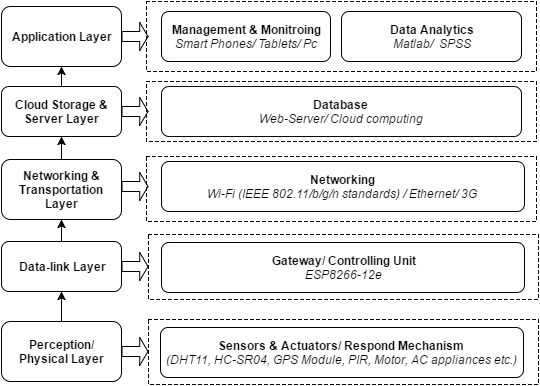
\includegraphics[width=3.0in]{figure1}
\caption{IoT Architecture of the Project}
\label{fig:artchitecture}
\end{figure}

\section{Hardware Design}
The system is divided into two major parts: software and
hardware design. Hardware configuration involves arranging
microprocessor, microcontroller, sensors and actuators whereas
software portion encloses programming that is written and
uploaded in each of the microcontrollers and microprocessor.

The system consists of microcontroller connected to sensors
and electrical devices that are to be monitored and controlled.
This section shows how different hardware components are set
up. The specifications and information regarding various
components used in this system are descriptively explicated
below.

\begin{figure}[!t]
\centering
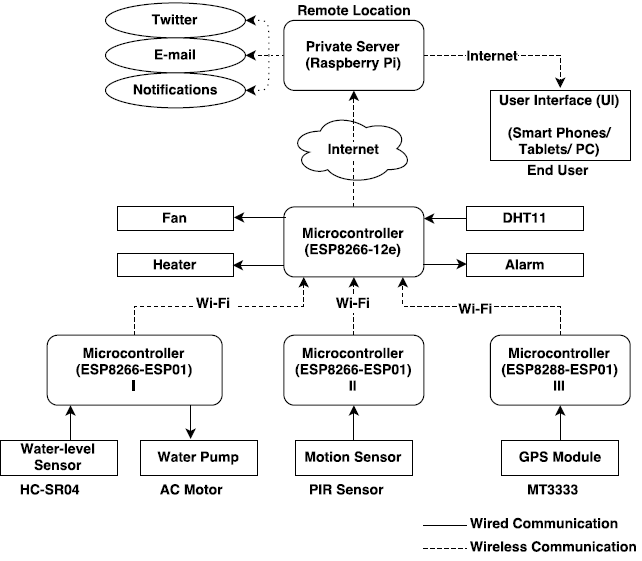
\includegraphics[width=3.0in]{figure2}
\caption{Schematic Plan of the Project}
\label{fig:schema}
\end{figure}

\subsection{Microprocessor Unit (CPU) – Raspberry pi}
The Raspberry Pi is a series of credit card-sized single-board
computers developed in the United Kingdom by the Raspberry
Pi Foundation with the intent to promote the teaching of basic
computer science in schools and developing countries. 

Raspberry pi 2 is a 900MHz quad-core ARM Cortex-A7
CPU with 1GB RAM. It consists of 4 USB ports, 40 GPIO pins,
Full HDMI port, Ethernet port, combined 3.5mm audio jack and
composite video, camera interface (CSI), Display interface
(DSI), micro SD card slot and a video-core IV 3D graphics core.
It has an ARMv7 processor and hence it can run the full range of
ARM GNU/Linux distributions, including Ubuntu Core, as well
as Microsoft Windows 10. SD cards are used to store the
operating system and program memory in either the SDHC or
MicroSDHC sizes. Lower level output is provided by a number
of GPIO pins which support common protocols like I2C.


\subsection{Microcontroller Unit (MCU) - ESP8266}
The ESP8266 is a low-cost Wi-Fi chip with full TCP/IP stack
and microcontroller capability produced by Shanghai-based
Chinese manufacturer i.e. Espressif \cite{Espressif2016}. The chip first came to
the attention of western makers in August 2014 with the ESP-01
module, made by a third-party manufacturer - AI-Thinker. This
small module allows microcontrollers to connect to a Wi-Fi
network and make simple TCP/IP connection using Hayes-style
commands.

ESP8266EX requires minimal external circuitry and
integrates a 32-bit Tensilica MCU, standard digital peripherals
interfaces, PCB traced antennal, RF balun, power amplifier, low
noise receive amplifier, filters and power management modules;
running at 80MHz. It consists of 64 KiB of instruction RAM,
and 96KiB of data RAM. It does have up to 16 GPIO pins and
advocates SPI as well as I2C communication networking \cite{Espressif2016}. It
is ultra-low power consuming device with ample processing
speed.

\subsection{Sensor Units}
A myriad number of sensors are being used in this system to
measure various parameters of environment. The system
decisions and operations are controlled by the sensors’ readings.

Ambient temperature and humidity is measured by DHT11
sensor, water-level in tank is incessantly measured by ultrasonic
sensor, motion is detected by IR sensor and path/ location of a
remote vehicle is tracked by a GPS sensor.

\subsection{User Interface}
The graphical interfaces in smart phones and tablets are
designed in the form of android and iOS applications by putting
buttons, graph-plotter, LCD and sensor-value display. The user
can simply download the app, log in and then monitor and
control her entire home appliances. The interface should enable
the user to look at the device status and regulate them.

Similarly, UI embodies a web portal for inspecting the status
and controlling them from desktop PCs and laptops. Web portal
is designed by making webpages from where the user can log in
and access the status of her entire home appliances and control
them through desktop PCs.

\section{Working of the System}

The system consists of three isolated sub-systems: first sub-
system consisting of GPS module to get the geo-location, second
sub-system consisting of multiple sensors – DHT11 temperature
sensor to measure temperature, PIR sensor to detect motion and
ultrasonic sensor to measure the distance, and the third sub-
system consisting of a master microcontroller which function as
the central coordinator that communicates with other subsystems
via Wi-Fi. The master microcontroller is also interfaced with a
relay module to control the appliances at the site. The sensor data
are fetched to the user interface facilitated by smartphones or
tablets from the various sensors using a raspberry pi as the
private server.

Basically, control of turning ON or OFF the whole system is
at owner’s hand. As the system gets powered up, it searches for
the preset SSID (Service Set Identifier) and connects
automatically to the Internet otherwise remains offline and
performs the automated-controlling job that doesn't require
commands from the owner.

\begin{figure}[!t]
\centering
\includegraphics[width=3.0in]{figure3}
\caption{Working Plan of the Proposed System}
\label{fig:working}
\end{figure}

Sensors accumulate disparate ambient-conditions and
transmit them to the Microcontroller which processes the data
transmitted by each sensor separately and then concurrently send
the acquired data to the web server. The readings of each sensor
can be accessed by the user from any place at any time.
Additionally, all the sensors’ data are logged per second for
future data analysis purpose. Data-logging is done both in
microSD card and in the server.

The system operates in two modes – automatic mode and
manual mode. When it is set at automatic mode, all the home
appliances like fan, heater etc. are automated to operate as per
the surrounding environmental conditions sensed by the sensors.
On the other hand, when it is set at manual mode, the user can
locally or remotely monitor and control each of the home
appliances via her smart phone or from her office-desktop PC.
To recapitulate, the surveillance and control of entire household
appliances is under her finger tip.

Beyond auto-manual mode of operation, some of the
activities like regular water level (in water-storage tank)
inspection and turning ON or OFF the water pump, ringing
alarms when detecting human-presence at the door which can
also be used for security by installing the motion detectors on
home or office so as to alert owner remotely. The user doesn’t
need to switch these devices at regular interval as they are self-
run under the commands of the microcontroller continuously
round the clock.

Similarly, some of the alert signals and warnings like house
on fire, gas leakage, intruders’ detection etc. are wirelessly
conveyed and notified about the situation to the house owner via
e-mail and phone notification. Using GPS, the owner can track
and locate her car at any moment from anywhere. To sum up,
IoT provides greater extent of security- physical as well
psychological.

\section{Results and Applications}

The proposed prototype of the system was designed and
exhibited on the 13th National Technological Festival, Locus-
2016, Pulchowk campus, Nepal.

\begin{figure}[!b]
    \begin{minipage}[t]{.45\linewidth}
        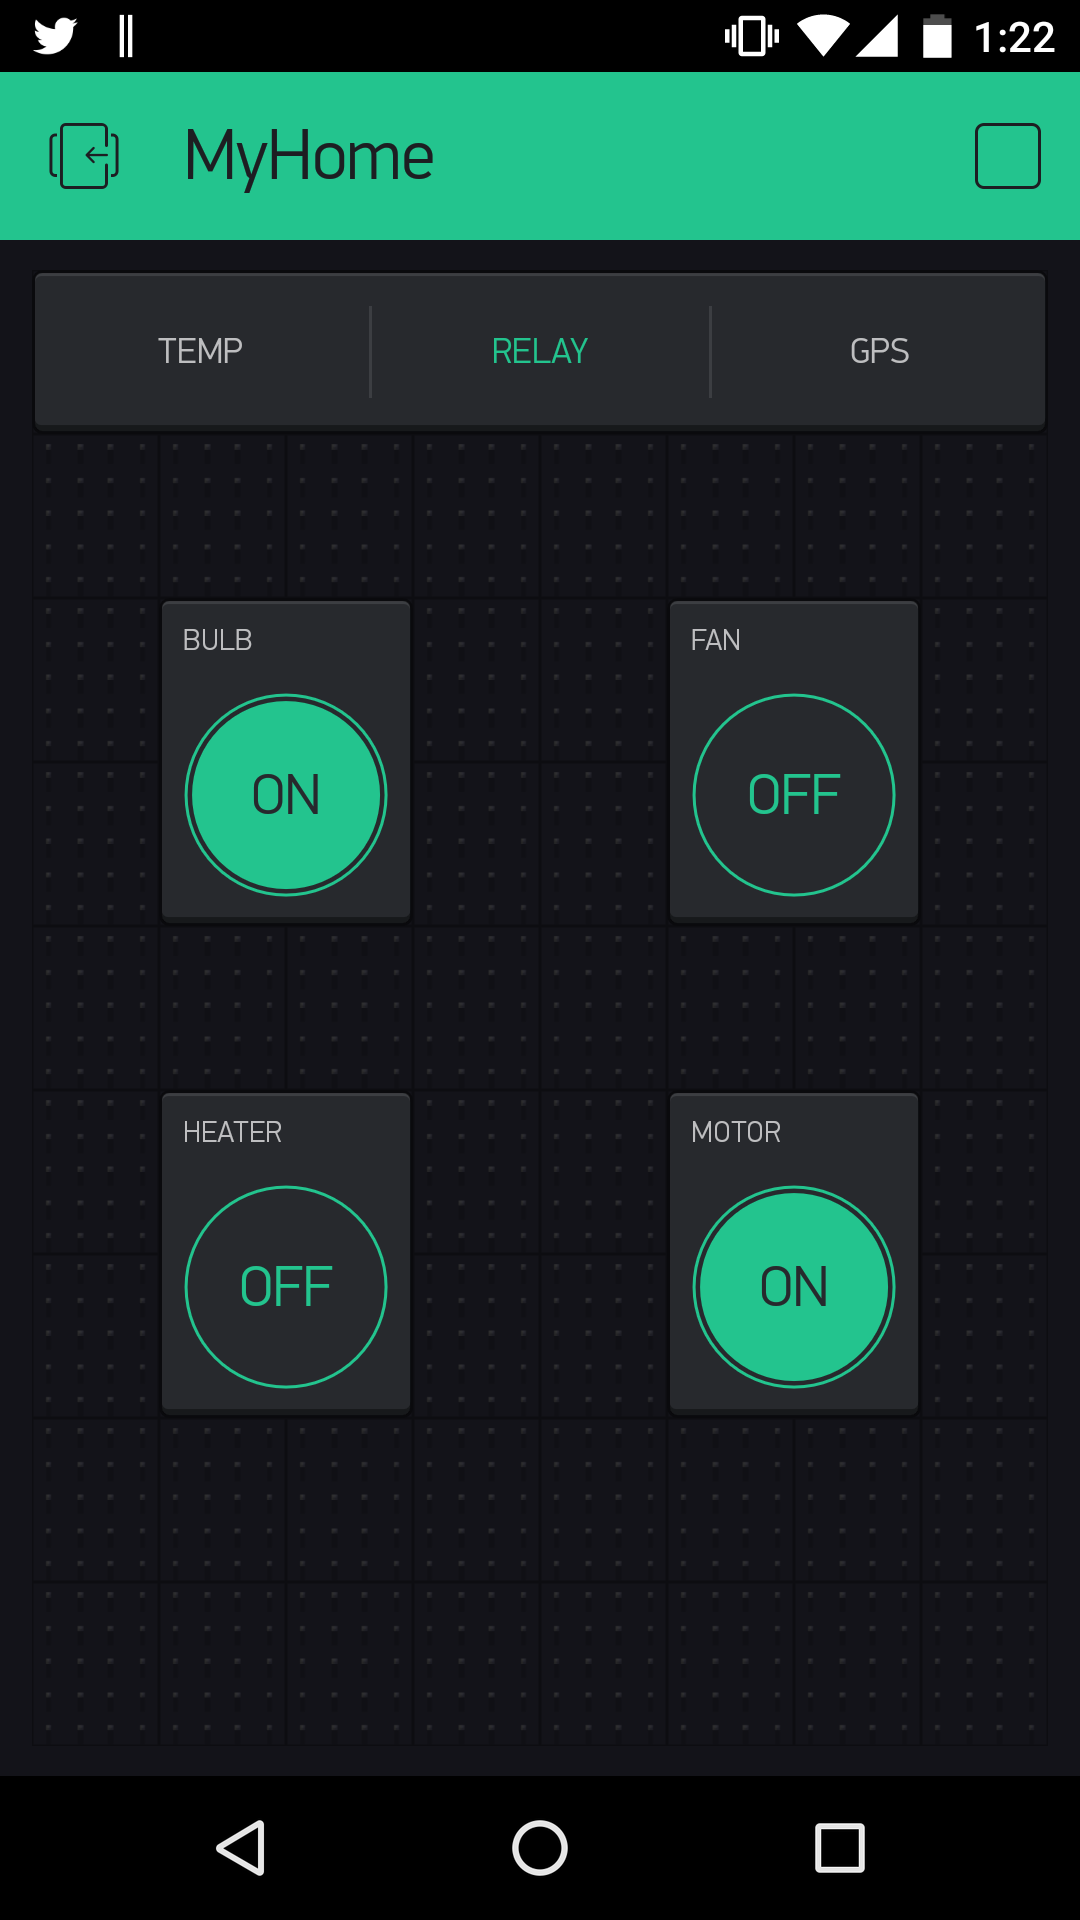
\includegraphics[width=\linewidth]{figure4a}
    \end{minipage}%
        \hfill%
    \begin{minipage}[t]{.45\linewidth}
        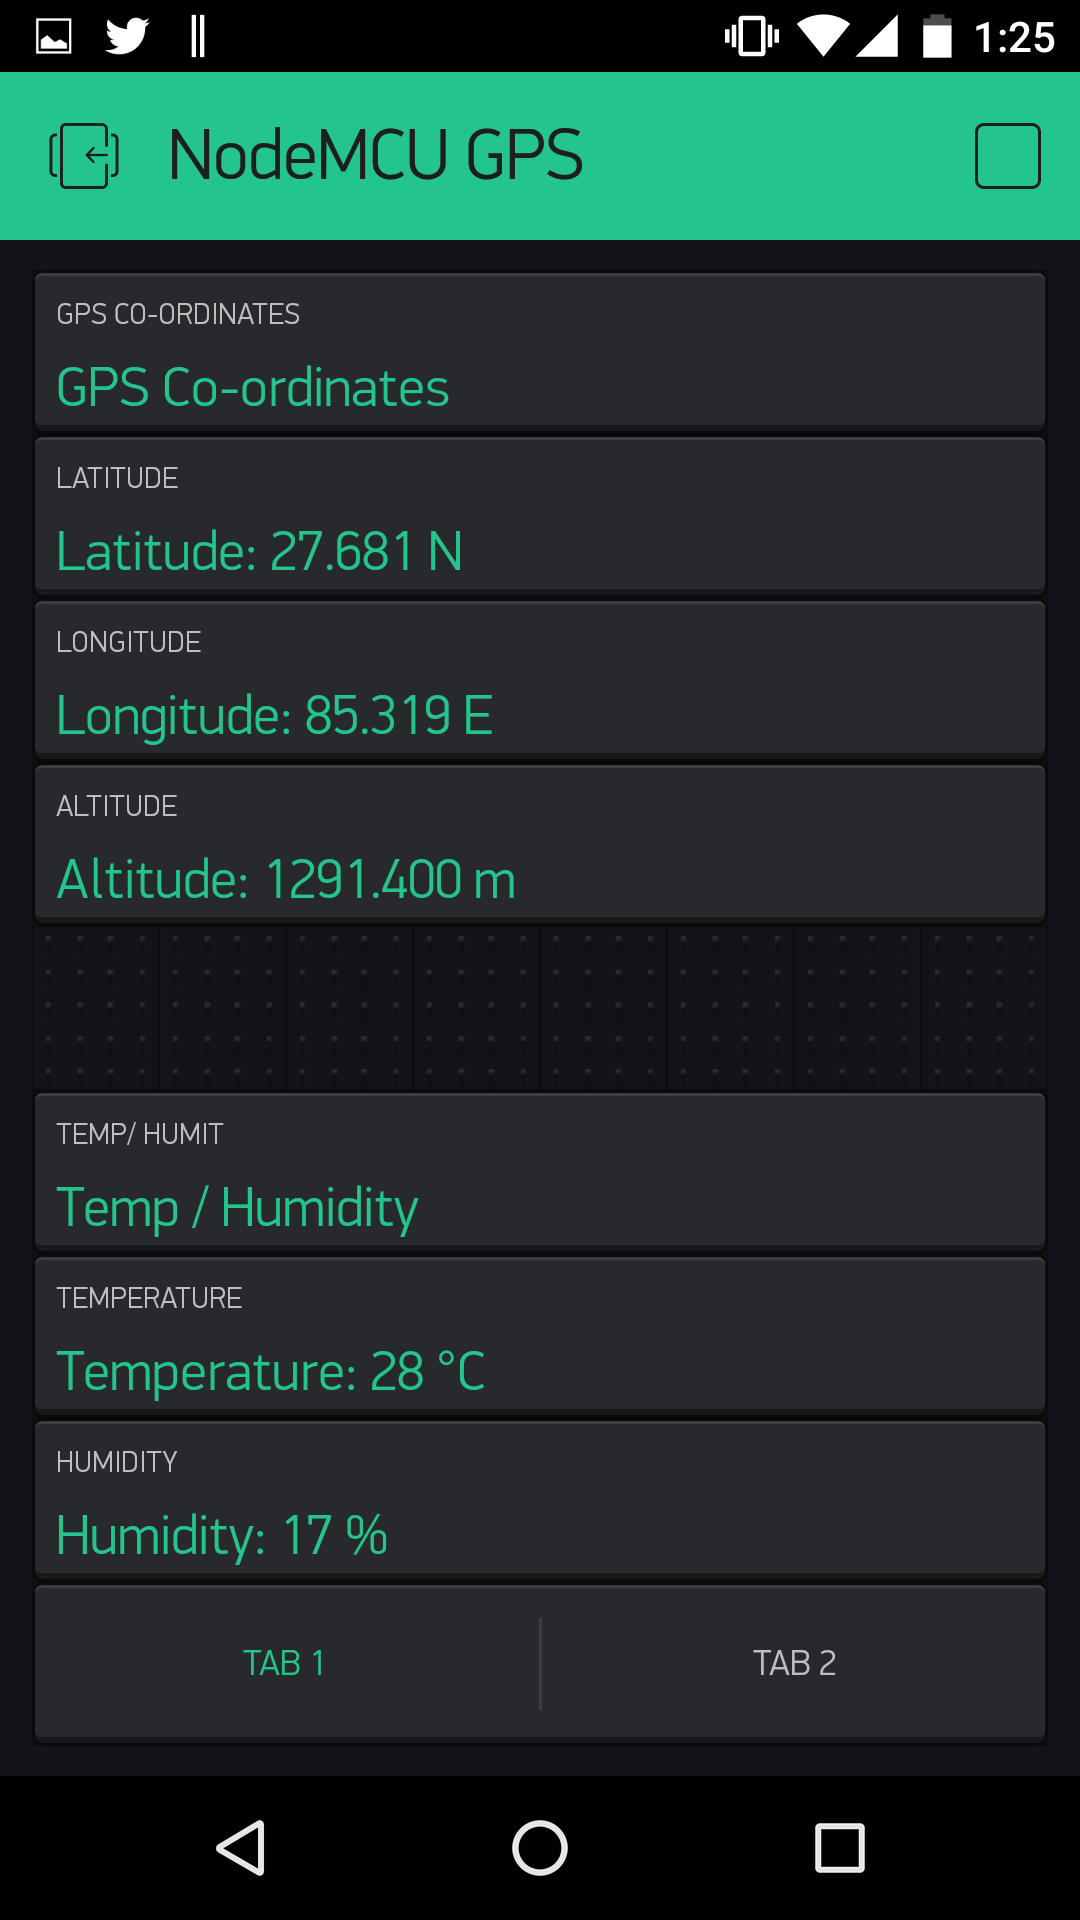
\includegraphics[width=\linewidth]{figure4b}
    \end{minipage}%
    \caption{Screenshots showing appliance switches and sensor outputs}
    \label{fig:Screenshot1}
\end{figure}

Three different isolated sub-systems : i) relay module system
connected to the home appliances to be controlled ii) GPS
module and Temperature sensor connected system iii) PIR
sensor for motion detection and ultrasonic senor for measuring
the water level in the tank were linked to one another via Wi-Fi
using NodeMcu controller chip. For user interface, android
version of Blynk app with custom designed layout and buttons
was used to facilitate monitoring and controlling various
connected things.

The screenshots of the results of the designed system
obtained on android application are shown in Figure~\ref{fig:Screenshot1}.

%\begin{figure*}[!t]
%    \begin{subfigure}[t]{.5\textwidth}
%        \centering
%        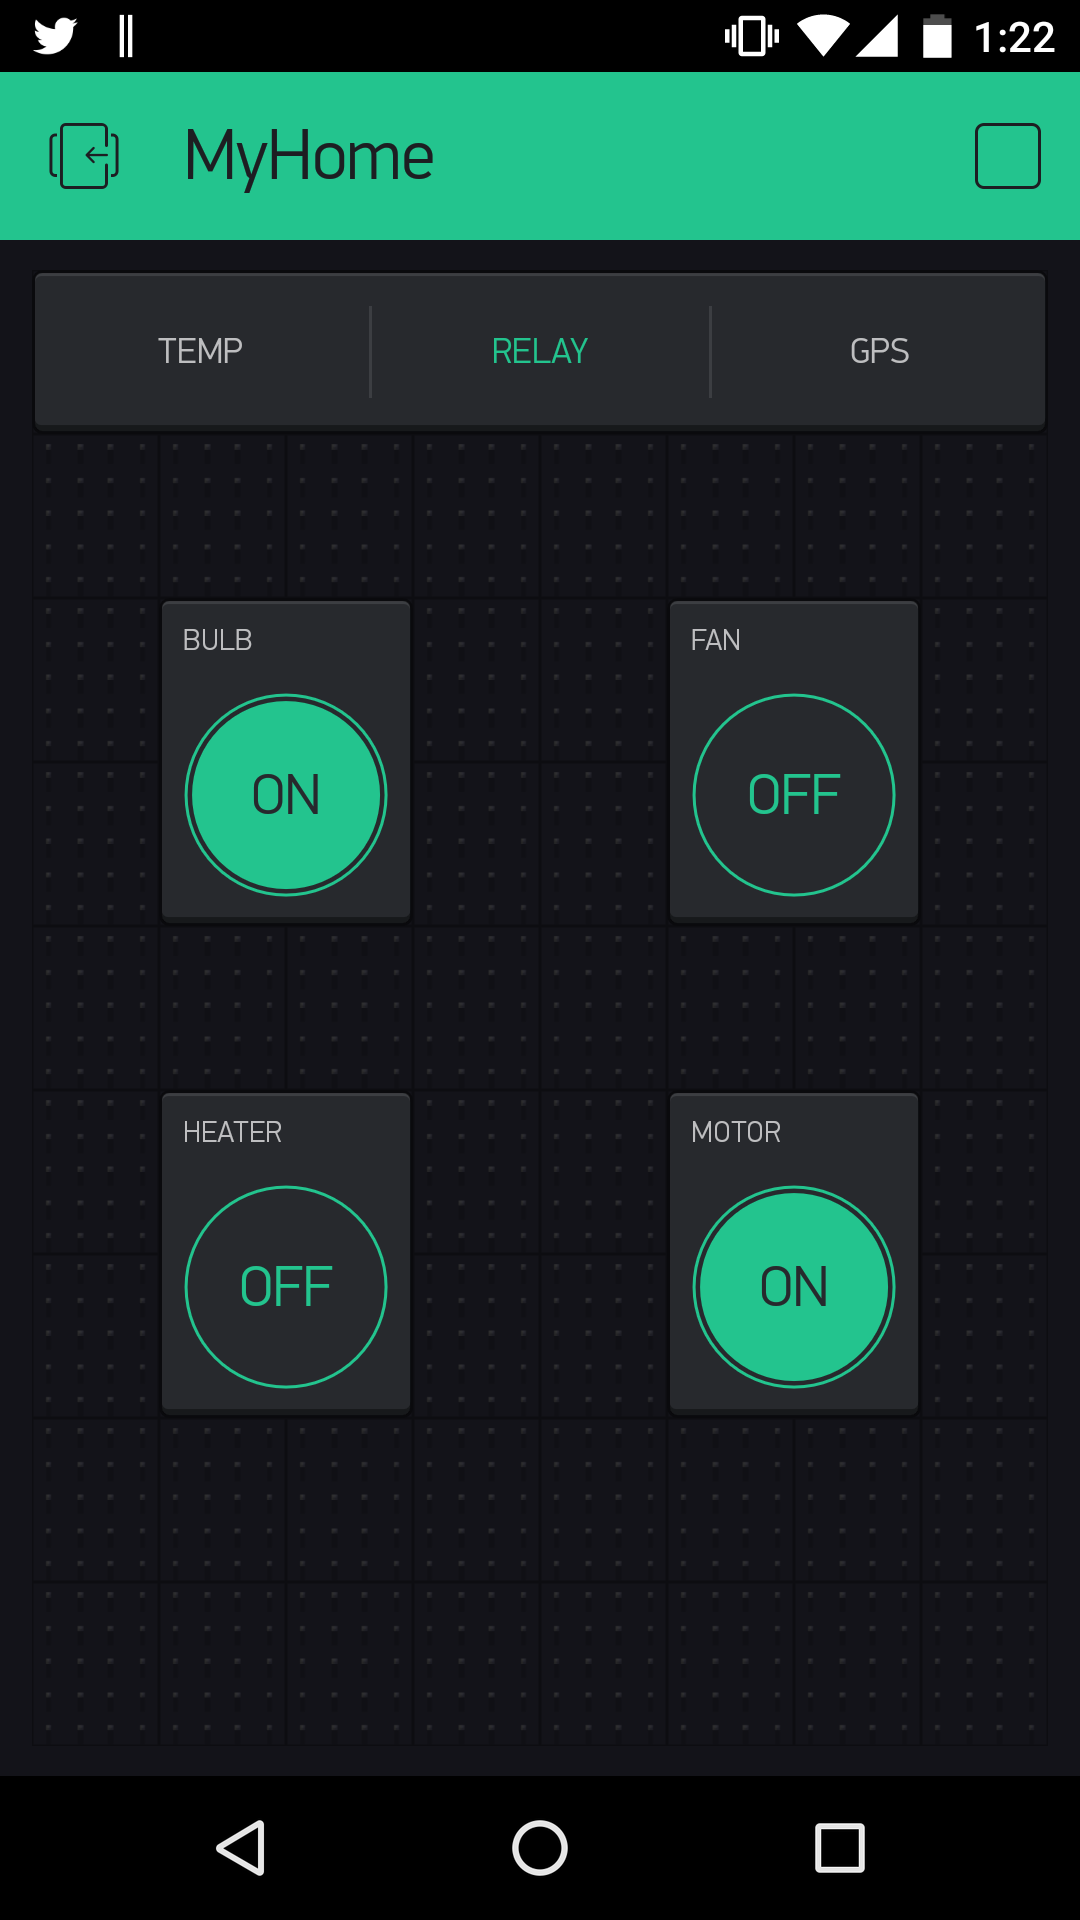
\includegraphics[width=50pt]{figure4a}
%        %\label{fig:sub1}
%    \end{subfigure}%
%    \begin{subfigure}[t]{.5\textwidth}
%        \centering
%        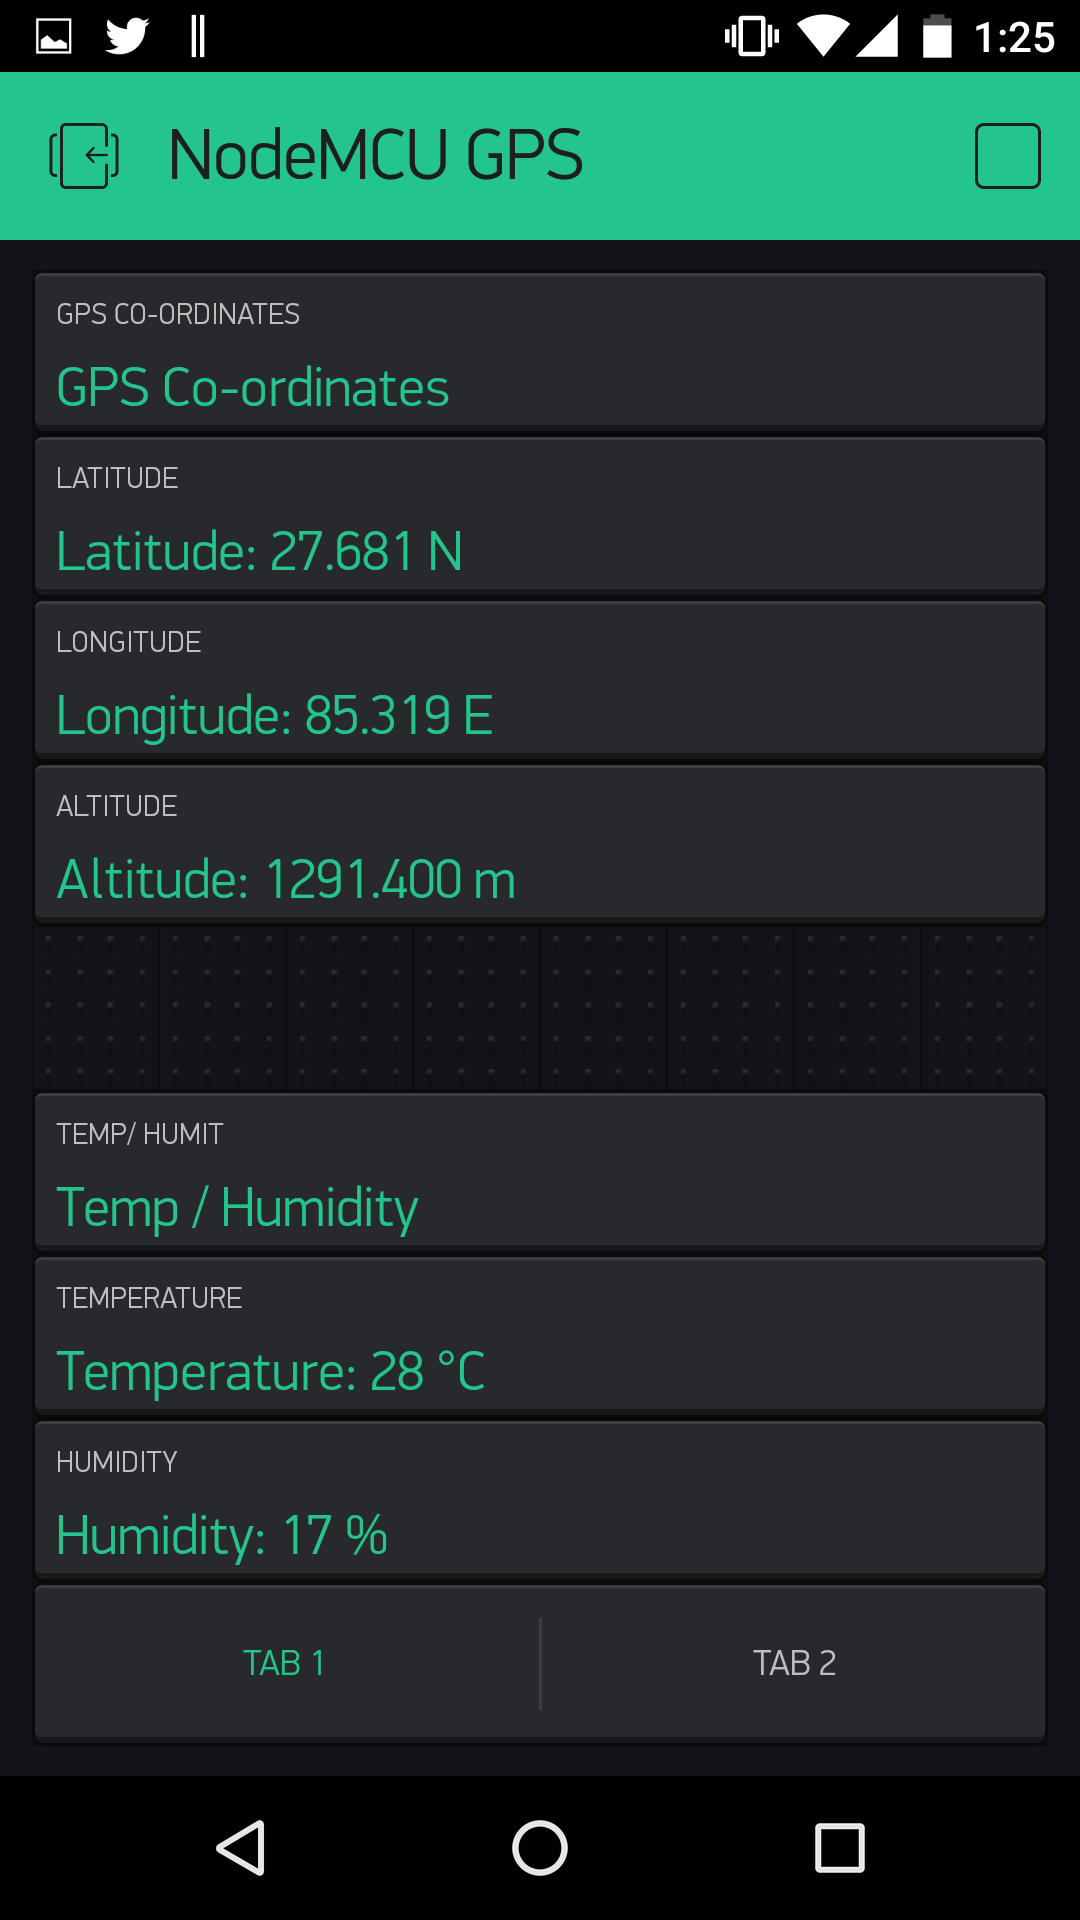
\includegraphics[width=50pt]{figure4b}
%        %\label{fig:sub2}
%    \end{subfigure}
%    \caption{Screenshots of switches for appliances and sensor data.}
%    \label{Screenshot1}
%\end{figure*}


By pressing virtual button on the smartphone, the home
appliances can be controlled from any remote location. One
advantage of this app is that it can be shared within all the family
members of the house. When one member switches ON or OFF
an appliance, the action will be apparent to all other members
sharing the app. Similarly, real-time as well as historical data of
measurements of temperature, humidity, GPS location and
distance-measure can be obtained from anywhere using the app.

Further, this system can be employed in many places such as
banks, hospitals, laboratories, traffic stations, residential
apartments, house, streets, poultry farms, greenhouse etc. In a
nutshell, this system can be used at multiple fields and areas in
order to make them operate “smartly”.

\begin{figure}[H]
\centering
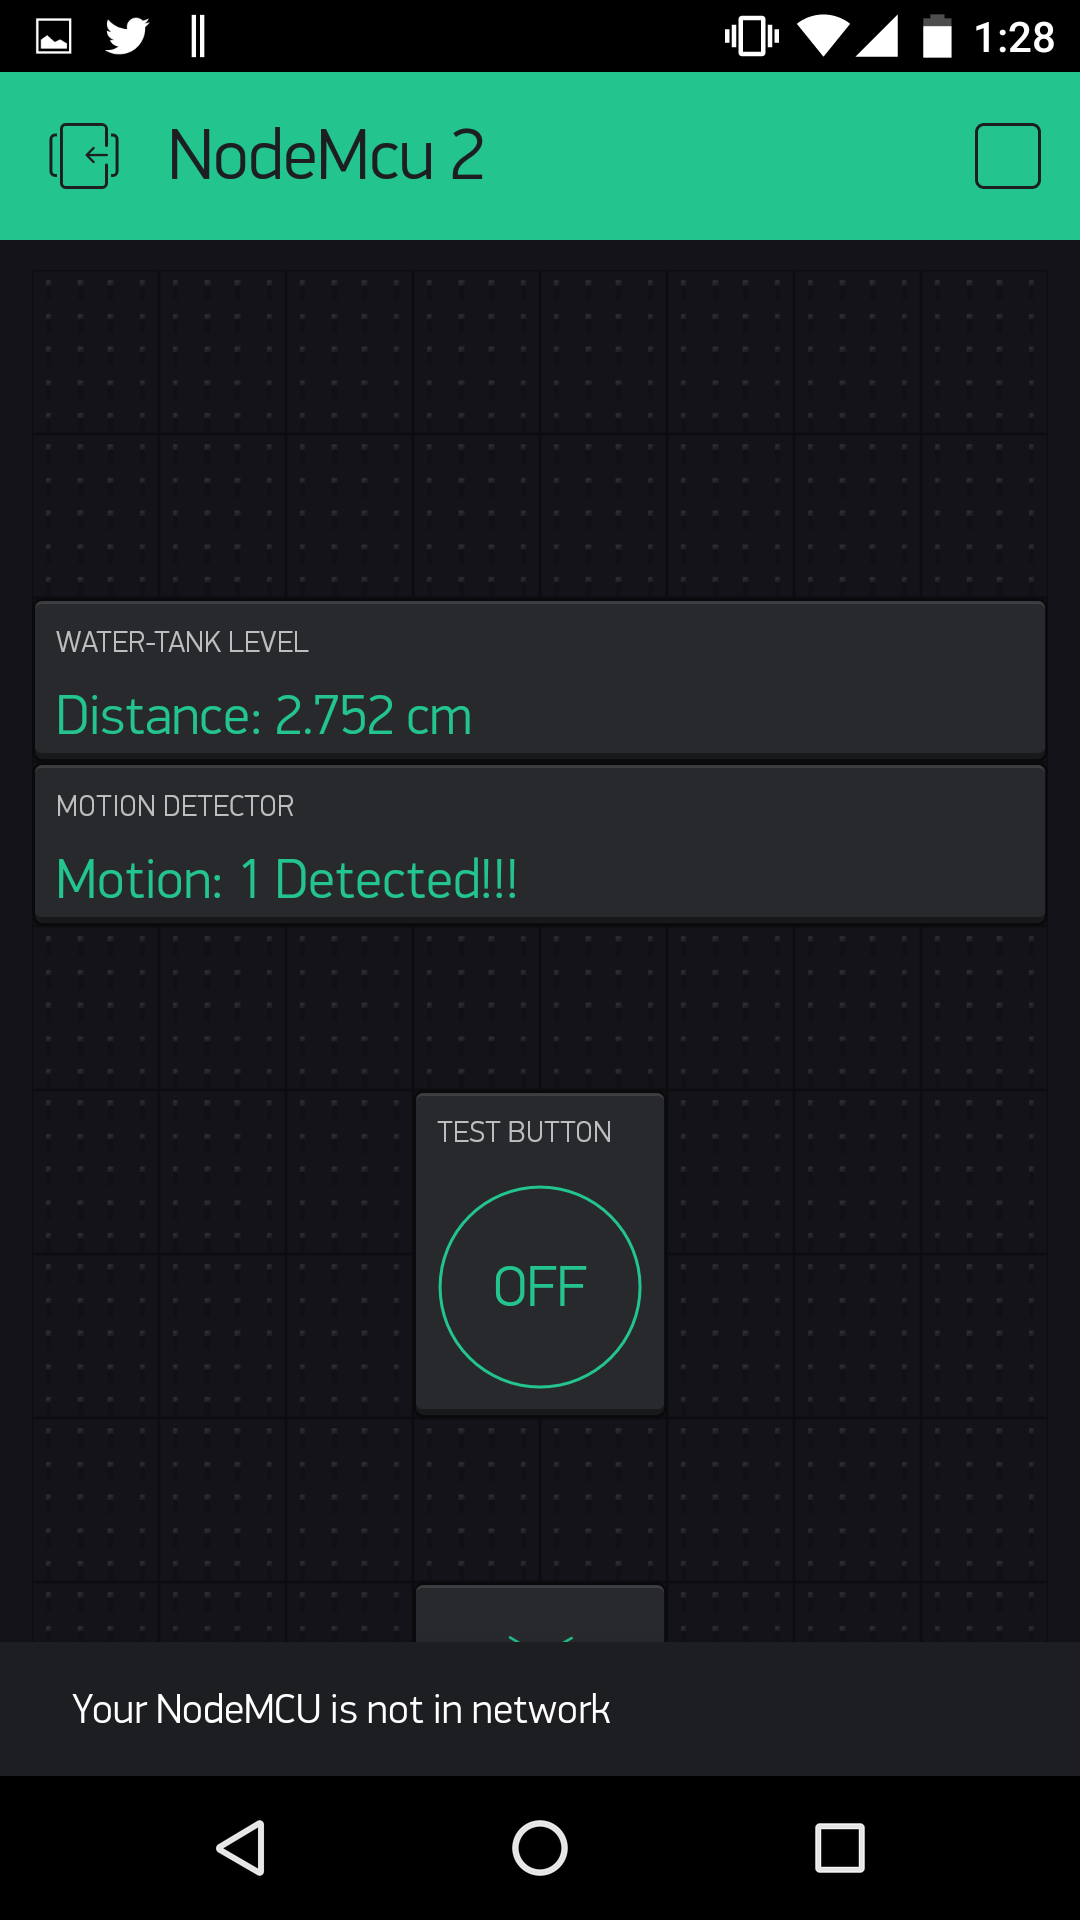
\includegraphics[width=2.0in]{figure5}
\caption{Screenshots showing distance measured and motion detected.}
\label{fig:Screenshot2}
\end{figure}

% needed in second column of first page if using \IEEEpubid
%\IEEEpubidadjcol

% An example of a floating figure using the graphicx package.
% Note that \label must occur AFTER (or within) \caption.
% For figures, \caption should occur after the \includegraphics.
% Note that IEEEtran v1.7 and later has special internal code that
% is designed to preserve the operation of \label within \caption
% even when the captionsoff option is in effect. However, because
% of issues like this, it may be the safest practice to put all your
% \label just after \caption rather than within \caption{}.
%
% Reminder: the "draftcls" or "draftclsnofoot", not "draft", class
% option should be used if it is desired that the figures are to be
% displayed while in draft mode.
%
%\begin{figure}[!t]
%\centering
%\includegraphics[width=2.5in]{myfigure}
% where an .eps filename suffix will be assumed under latex, 
% and a .pdf suffix will be assumed for pdflatex; or what has been declared
% via \DeclareGraphicsExtensions.
%\caption{Simulation Results}
%\label{fig_sim}
%\end{figure}

% Note that IEEE typically puts floats only at the top, even when this
% results in a large percentage of a column being occupied by floats.


% An example of a double column floating figure using two subfigures.
% (The subfig.sty package must be loaded for this to work.)
% The subfigure \label commands are set within each subfloat command, the
% \label for the overall figure must come after \caption.
% \hfil must be used as a separator to get equal spacing.
% The subfigure.sty package works much the same way, except \subfigure is
% used instead of \subfloat.
%
%\begin{figure*}[!t]
%\centerline{\subfloat[Case I]\includegraphics[width=2.5in]{subfigcase1}%
%\label{fig_first_case}}
%\hfil
%\subfloat[Case II]{\includegraphics[width=2.5in]{subfigcase2}%
%\label{fig_second_case}}}
%\caption{Simulation results}
%\label{fig_sim}
%\end{figure*}
%
% Note that often IEEE papers with subfigures do not employ subfigure
% captions (using the optional argument to \subfloat), but instead will
% reference/describe all of them (a), (b), etc., within the main caption.


% An example of a floating table. Note that, for IEEE style tables, the 
% \caption command should come BEFORE the table. Table text will default to
% \footnotesize as IEEE normally uses this smaller font for tables.
% The \label must come after \caption as always.
%
%\begin{table}[!t]
%% increase table row spacing, adjust to taste
%\renewcommand{\arraystretch}{1.3}
% if using array.sty, it might be a good idea to tweak the value of
% \extrarowheight as needed to properly center the text within the cells
%\caption{An Example of a Table}
%\label{table_example}
%\centering
%% Some packages, such as MDW tools, offer better commands for making tables
%% than the plain LaTeX2e tabular which is used here.
%\begin{tabular}{|c||c|}
%\hline
%One & Two\\
%\hline
%Three & Four\\
%\hline
%\end{tabular}
%\end{table}


% Note that IEEE does not put floats in the very first column - or typically
% anywhere on the first page for that matter. Also, in-text middle ("here")
% positioning is not used. Most IEEE journals use top floats exclusively.
% Note that, LaTeX2e, unlike IEEE journals, places footnotes above bottom
% floats. This can be corrected via the \fnbelowfloat command of the
% stfloats package.



\section{Conclusion and Future Works}

In this paper, we have introduced a home management
and security system. This paper is mainly focused on 
overcoming everyday problems faced by the people in
Nepal where regular power cut-off, unmanaged
urbanization, lack of manpower in agriculture and
farming, etc are blatantly evident. Our prototypical system
is applicable to real-time home security, automation,
monitoring and controlling of remote systems.

The future works include: 1) Implementation of the project
in one of the remote parts of Nepal to collect data like wind
speed, solar irradiance etc. for future research 2) Feasibility
study and implementation of the project in an unmanaged and
polluted cities like Kathmandu 3) Application of the project in
residential complexes and small-scale industries \cite{Pavithra2015} \cite{Zuehlke2010} and
traditional greenhouses\cite{Dan2015}  4) Big data analytics on the collected
data using appropriate tools and techniques \cite{Signorini2016}.


% if have a single appendix:
%\appendix[Proof of the Zonklar Equations]
% or
%\appendix  % for no appendix heading
% do not use \section anymore after \appendix, only \section*
% is possibly needed

% use appendices with more than one appendix
% then use \section to start each appendix
% you must declare a \section before using any
% \subsection or using \label (\appendices by itself
% starts a section numbered zero.)
%


% \appendices
% \section{Proof of the First Zonklar Equation}
% Some text for the appendix.

% use section* for acknowledgement
\section*{Acknowledgment}

We would like to thank Asst. Prof. Dr. Arun K. Timalsina,
IOE, Pulchowk Campus, Tribhuvan University for guiding us
throughout this research project. We are also very much
thankful towards Blynk organization for granting us permission
to access its cloud server along with its resources and library
files.


% Can use something like this to put references on a page
% by themselves when using endfloat and the captionsoff option.
\ifCLASSOPTIONcaptionsoff
  \newpage
\fi



% trigger a \newpage just before the given reference
% number - used to balance the columns on the last page
% adjust value as needed - may need to be readjusted if
% the document is modified later
%\IEEEtriggeratref{8}
% The "triggered" command can be changed if desired:
%\IEEEtriggercmd{\enlargethispage{-5in}}

% references section

% can use a bibliography generated by BibTeX as a .bbl file
% BibTeX documentation can be easily obtained at:
% http://www.ctan.org/tex-archive/biblio/bibtex/contrib/doc/
% The IEEEtran BibTeX style support page is at:
% http://www.michaelshell.org/tex/ieeetran/bibtex/
%\bibliographystyle{IEEEtran}
% argument is your BibTeX string definitions and bibliography database(s)
%\bibliography{IEEEabrv,../bib/paper}
%
% <OR> manually copy in the resultant .bbl file
% set second argument of \begin to the number of references
% (used to reserve space for the reference number labels box)
\begin{thebibliography}{99}

    \bibitem{Blynk2016}
        "Home", \emph{Blynk}. [Online]. Available: http://www.blynk.cc/. [Accessed: 23-May-2016].

    \bibitem{Floerkemeier2008}
        C. Floerkemeier et al. (eds.), "The Internet of Things" in \emph{First International Conference, IOT 2008, Zurich, Switzerland, March 26-28, 2008, Proceedings.} 
        Vol. 4952. Springer, 2008.

    \bibitem{NEA2016}
        L.Paudel, "Loadshedding Schedule," \emph{Nepal Electricity Authority}. [Online]. Available: http://nea.org.np/loadshedding.html. [Accessed: 16- May- 2016].

    \bibitem{Dan2015}
        L.Dan et al., "Intelligent Agriculture Greenhouse Environment Monitoring System Based on IOT Technology." 
        in \emph{2015 International Conference on Intelligent Transportation, Big Data and Smart City (ICITBS)}, 
        pp. 487-490. IEEE, 2015.

    \bibitem{Zeng2011}
        D. Zeng, S. Guo, and Z. Cheng, “The Web of Things: A Survey (Invited Paper),” Journal of Communications, vol. 6, no. 6, Jan. 2011.

    \bibitem{Raul2014} 
        R.Garcıa-Castro, A. Gómez-Pérez, and O. Corcho
        "Ready4Smartcities: ICT roadmap and data interoperability for energy systems in smart cities", 
        in \emph{11th Extended Semantic Web Conference (ESWC’14).}, 2014.


    \bibitem{Lecue2014}
        F. Lecue et al.
        "Star-city: semantic traffic analytics and reasoning for city", 
        in \emph{Proceedings of the 19 th International Conference on Intelligent Users Interfaces.} 
        ACM, 2014, pp. 179-188

    \bibitem{Barnaghi2014}
        P. Barnaghi et al., 
        "Citypulse: Real-time IoT Stream Processing and Large-scale data analytics for smart city applications", 
        in \emph{2014 European Semantic Web Conference}, 2014.

    \bibitem{Sanchez2011}
        L. Sanchez et al.,
        "Smartsantander: The metting point between future internet research and experimentation and the smart cities", 
        in \emph{Future Network \& Mobile Summit, 2011, IEEE}, 2011, pp. 1-8

    \bibitem{Espressif2016}
        "Espressif Systems - Wi-Fi and Bluetooth chipsets and solutions", \emph{Espressif.}. [Online]. Available: https://espressif.com/. [Accessed: 27- May- 2016].

    \bibitem{Pavithra2015}
       D. Pavithra and R. Balakrishnan, 
       “IoT based monitoring and control system for home automation,” 
       \emph{2015 Global Conference on Communication Technologies (GCCT)}, 2015. 

    \bibitem{Zuehlke2010}
       D. Zuehlke, 
       “SmartFactory—Towards a factory-of-things,” 
       \emph{Annual Reviews in Control}, vol. 34, no. 1, pp. 129–138, 2010. 

    \bibitem{Signorini2016}
        E. Signorini, 
        "Solving Advanced IoT Analytics with the Databricks Just-in-time Appraoach", 2016. [Online]. Available: http://go.databricks.com/solving-advanced-iot-analytics-with-the- databricks-just-in-time-approach. [Accessed: 27- May- 2016].


\end{thebibliography}

% biography section
% 
% If you have an EPS/PDF photo (graphicx package needed) extra braces are
% needed around the contents of the optional argument to biography to prevent
% the LaTeX parser from getting confused when it sees the complicated
% \includegraphics command within an optional argument. (You could create
% your own custom macro containing the \includegraphics command to make things
% simpler here.)
%\begin{biography}[{\includegraphics[width=1in,height=1.25in,clip,keepaspectratio]{mshell}}]{Michael Shell}
% or if you just want to reserve a space for a photo:

% You can push biographies down or up by placing
% a \vfill before or after them. The appropriate
% use of \vfill depends on what kind of text is
% on the last page and whether or not the columns
% are being equalized.

%\vfill

% Can be used to pull up biographies so that the bottom of the last one
% is flush with the other column.
%\enlargethispage{-5in}

\newpage
\begin{IEEEbiography}[{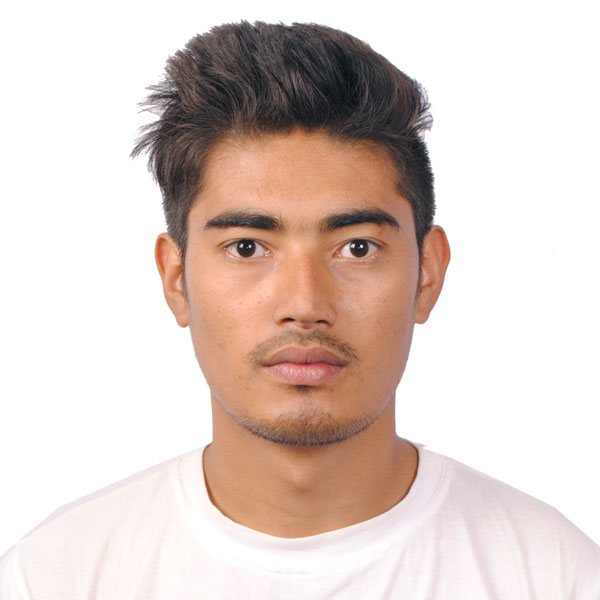
\includegraphics[width=1in,height=1.25in,clip,keepaspectratio]{bharat}}]{Bharat Bohara}
    received B.E. degree in Electrical and Electronics Engineering from Kathmandu University, Dhulikhel, Nepal, in 2015. His research interests include clean and renewable energy, Information and Communication Technology (ICT), and rural electrification. Currently, he is working at District Development Committee (DDC), Humla as a district energy officer deployed by Alternative Energy Promotion Centre (AEPC), Nepal.
\end{IEEEbiography}
\vspace{-12cm}
\begin{IEEEbiography}[{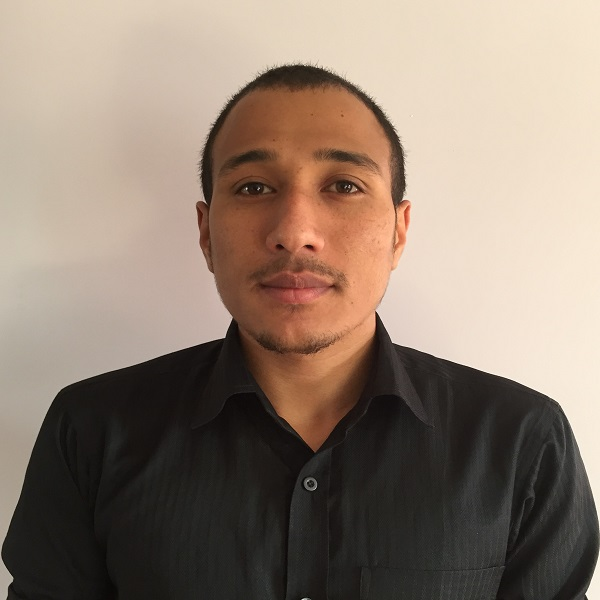
\includegraphics[width=1in,height=1.25in,clip,keepaspectratio]{sunil}}]{Sunil Maharjan}
    received B.E. degree in Mechanical Engineering from Kathmandu University, Dhulikhel, Nepal, in 2015. He is currently working as Network Manager at CG|Motocorp with past experiences in research, 3D design and programming tools at E\&T. His research interests are energy optimization, 3D design, and industrial engineering.
\end{IEEEbiography}
\vspace{-12cm}
\begin{IEEEbiography}[{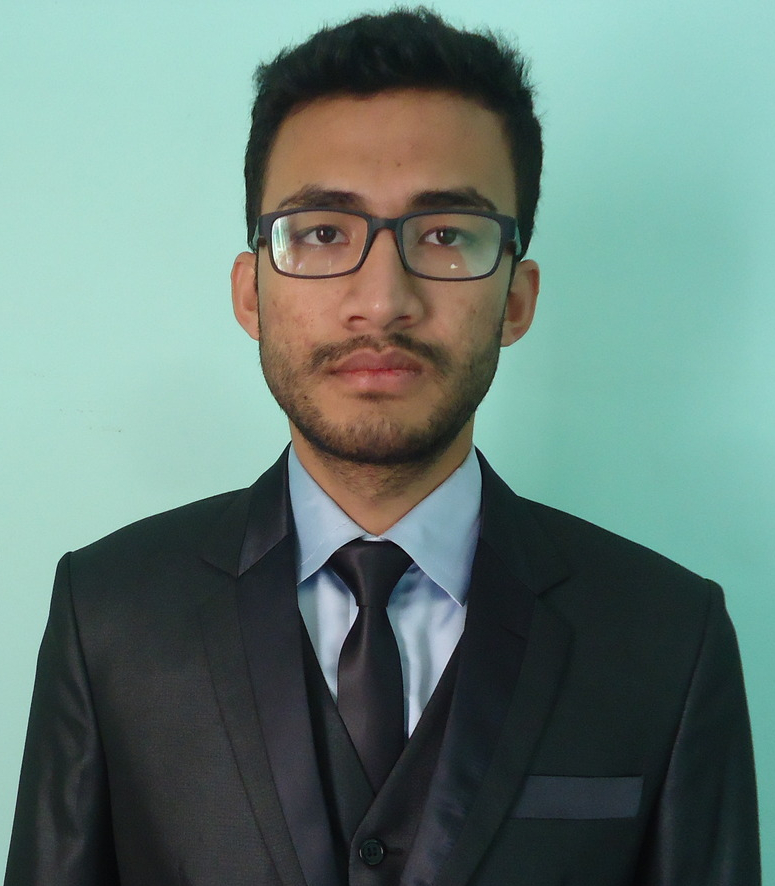
\includegraphics[width=1in,height=1.25in,clip,keepaspectratio]{bibek}}]{Bibek Raj Shrestha}
    is a fourth year computer engineering student at IoE, Pulchowk Campus, Lalitpur, Nepal. His research interests are in the areas of Data Management, and Distributed Computing and Optimization. Currently, he is working as an offshore Intern at a big data innovation group - DR2Services Inc., MA, USA. His hobbies include hiking and traveling to new places.
\end{IEEEbiography}


% that's all folks
\end{document}


